\section{Speculation-Aware Scheduling Mechanism}
\label{sec:system}

While the Verified Speculation Phase reduces agent latency by overlapping reasoning and action execution, it introduces additional challenges in online serving scenarios. 
First, the additional speculative requests increase the computational load, potentially degrading overall inference speed. 
Second, inefficient scheduling between speculative and main agent requests can cause speculative action generation to finish later than the corresponding main agent requests. 
Such delays nullify the benefits of parallel execution. 
To address these challenges, we design a two-level scheduling framework: 
\textbf{Intra-Speculation Request Scheduling} dynamically regulates the emission of speculative requests to control inference overhead, and \textbf{Inter-Request Scheduling} globally prioritizes requests to ensure timely speculative completion.

\begin{figure}[t]
    \begin{subfigure}[c]{0.45\linewidth}
        \centering
        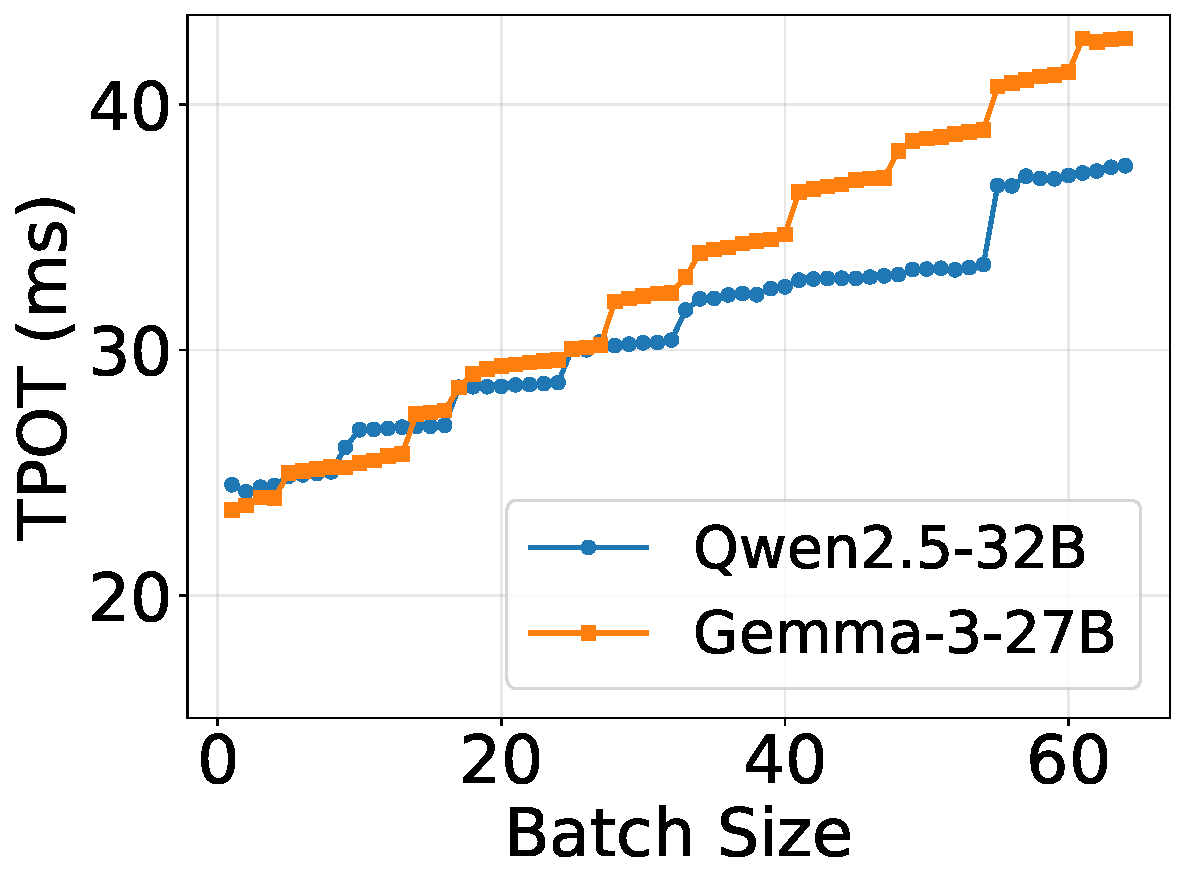
\includegraphics[width=\linewidth]{figures/experiments/batch_size_plots_tpot.pdf}
    \end{subfigure}
    \hfill
    \begin{subfigure}[c]{0.45\linewidth}
        \centering
        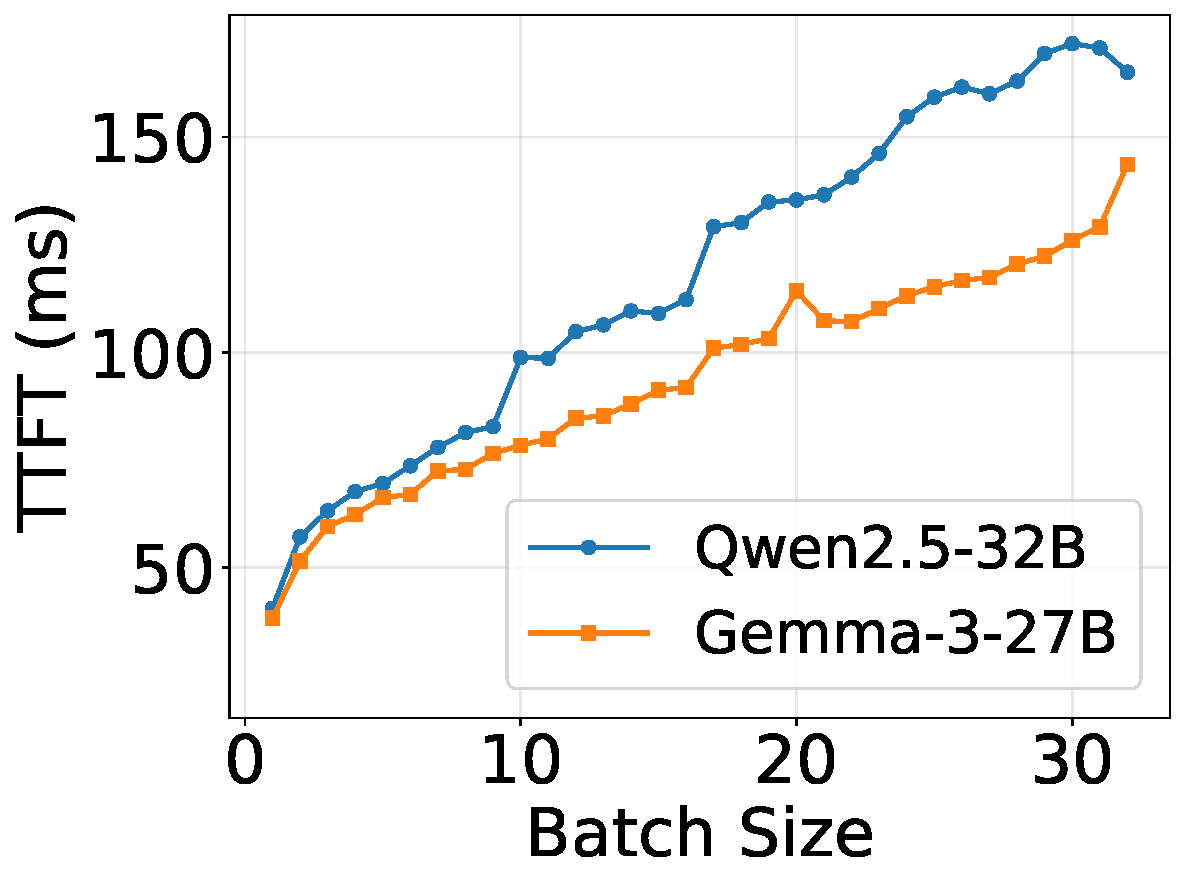
\includegraphics[width=\linewidth]{figures/experiments/batch_size_plots_ttft.pdf}
    \end{subfigure}
    % \vspace{-10pt}
    \caption{(a) Average TPOT and (b) Average TTFT on different batch sizes.}
    \label{fig:plots}
    % \vspace{-10pt}
\end{figure}

\subsection{Intra-Speculation Request Schedule}
\label{sec:intra-sched}

In the Verified Speculation Phase, speculative actions run concurrently with main agent reasoning to overlap tool latency, but they also introduce extra inference requests. 
Our profiling in \Figref{fig:plots}a and b shows that this overhead is negligible at low concurrency, as decode time remains stable and a single prefill request costs roughly one decode step. 
However, as concurrency increases, speculative requests inflate the number of active decode jobs, slowing per-step decode speed by around to 20\%. 
Moreover, batches begin to contain many prefill requests whose cost scales almost linearly with batch size, making hybrid batches several times more expensive than decode batch, thus blocking other ongoing requests.

These results indicate that speculative requests can easily outweigh their benefits under high load. 
This raises the key question: \emph{which} speculative requests should be launched, and \emph{how many}, so their expected latency reduction exceeds the added inference overhead.
To address this, we introduce the Intra-Speculation Request Schedule, which dynamically selects and emits speculative requests based on real-time engine load.


\begin{table}[t]
    \centering
    \small
    \caption{Notation used in the formulation.}
    % \vspace{-10pt}
    \setlength\tabcolsep{2pt} % default value: 6pt
    \footnotesize
    \begin{tabular}{ll}
        \toprule
        \textbf{Symbol} & \textbf{Meaning} \\
        \midrule
        $\mathcal{R}$ & Set of running main agent requests \\
        $S$ & Selected subset of $\mathcal{R}$ for speculation \\
        $k$ & Number of speculative samples per request \\
        $N$ & Total number of inference requests ($N_m{+}N_s{+}N_a$) \\
        $N_m$ & \# main agent inference requests ($|\mathcal{R}|$) \\
        $N_s$ & \# speculative inference requests (Verified Speculation phase) \\
        $N_a$ & \# inference requests from Aggressive phase \\
        $t_{act}$ & Average action execution time \\
        $p$ & Probability a speculative sample hits the correct action \\
        $l_s$ & Average speculative output length (tokens) \\
        $L_s$ & Input token length for speculative prefill \\
        $T_h(\cdot)$ & Engine profiling timing results for hybrid batches \\
        $T_{r,a}(S,N)$ & Expected latency reduction from overlap \\
        $T_{o,d}(S,N)$ & Decode phase overhead of speculative requests \\
        $T_{o,p}(S,N)$ & Prefill phase overhead of speculative requests \\
        \bottomrule
    \end{tabular}
    \label{tab:notion}
    % \vspace{-15pt}
\end{table}

The symbols used in our scheduling formulation are listed in \Tabref{tab:notion}.
Given the running main agent requests $\mathcal{R}$ in the Verified Speculation Phase, the scheduler selects a subset $S\subseteq\mathcal{R}$ to issue $k$ speculative samples.
The objective is to maximize the expected latency reduction minus inference overhead:
\begin{equation}
    \small
    \max_{S} T_r(S, N) = T_{r,a}(S, N) - (T_{o,d}(S, N)+T_{o,p}(S,N))
\end{equation}
For each $r\in S$, latency is reduced when at least one speculative sample matches the main agent action.
Under independent hit probability $p$, and suppose the action time can be fully overlapped by the main agent path, the expected reduction per task is:
\begin{equation}
    \small
    T_{r,a}(S, N) = \frac{1}{N_m + N_a}\sum_{r\in S} t_{act} \times [1-(1-p)^k]
\end{equation}

The overhead on the inference engine primarily manifests in the prefill and decode phases of speculative requests.
In widely-used engine like vLLM~\cite{vllm}, prefill requests are batched and computed with ongoing decode requests.
Considering the decode phase, speculation increases the number of concurrently processed requests, thereby raising the computational load per decode iteration, resulting in increasing time for one decode step.
Since speculative requests produce very short output length, typically fewer than ten tokens, we assume that the load of inference engine remains stable during each scheduling step.
So the overhead of decode phase is:
\begin{equation}
    \small
    T_{o,d}(S, N) = l_s \times (T_h(\emptyset, N+k\times |S|)-T_h(\emptyset, N))
\end{equation}
where $T_h(\emptyset, N)$ represents the computation time of a hybrid batch with no prefill requests and $N$ decode requests.

Prefill overhead is added once per speculative request, since all samples of one request share the same prefix:
\begin{equation}
    \small
    T_{o, p}(S, N) = T_h((L_s, |S|), N) - T_h(\emptyset, N)
\end{equation}
where $T_h((L_s, |S|), N)$ represents the computation time of a hybrid batch, including $|S|$ prefill requests with $L_s$ input tokens and $N$ decode requests.
% \begin{equation}
%     \small
%     T_{o}(S,N)=T_{o, p}(S) + T_{o,d}(S, N)
% \end{equation}
\begin{algorithm}[t]
\small
    \caption{Runtime Speculation Selection}
    \label{algo:intra-spec}
    \SetAlgoLined
    \SetKwData{Left}{left}\SetKwData{This}{this}\SetKwData{Up}{up}
    \SetKwFunction{FMain}{Speculation\_Select\_Step}
    \SetKwProg{Fn}{Function}{:}{}
    \SetKwInOut{Input}{Input}\SetKwInOut{Output}{Output}
    \Input{Speculation Priority Queue $Q_r$, Running Requests $N$}
    \Output{Speculation Choice $S$}
    \BlankLine
    \Fn{\FMain{$Q_r, N$}}{
        $S\leftarrow[\:]$\;
        $T_{r, best}\leftarrow 0$\;
        \While{$|Q_r|>0$}{
            $new\_spec\leftarrow Q_r$.pop() \# Candidate with highest priority\;
            \If{$new\_spec$.\text{wait\_time} > $t_w$}{\label{line:discard}
                Continue\;
            }
            $T_{r, cur}\leftarrow T_r(S + new\_spec, N)$\;
            \If{$T_{r, cur}>T_{r, best}$}{\label{line:accept}
                $T_{r, best}\leftarrow T_{r, cur}$\;
                $S$.append($new\_spec$)\;
            }
            \Else{
                Break\label{line:break}\;
            }
        }
        \Return $S$\;
    }
% \vspace{-10pt}
\end{algorithm}
% \vspace{-10pt}

At runtime, the scheduler maintains a priority queue that stores all main agent requests whose speculative actions have not yet been launched.
The priority of candidates is determined by two factors:
\begin{itemize}[leftmargin=*]
    \item First, the step index within the agent task: 
Requests from earlier steps are assigned higher priority, as earlier speculative actions have a higher probability of being adopted by the main agent, thus yielding greater benefit (as discussed in \Secref{sec:algo}).
    \item Second, the arrival time of requests: 
More recently arrived speculative requests are prioritized because they correspond to main agent path inferences that are farther from completion, leaving a longer window for parallel execution between speculative action and ongoing reasoning. 
To preserve this overlap, speculative requests that have waited beyond a predefined time threshold $t_w$ will be discarded, since their results would no longer provide meaningful parallelism or latency savings.
\end{itemize}


Using these two criteria, the scheduler greedily selects speculative requests to maximize the overall expected latency reduction under the current resource constraints of the inference engine.
As shown in \Algref{algo:intra-spec}, during each scheduling step, the scheduler repeatedly pops the highest-priority request from the queue and tentatively adds it to the speculative set $S$, accept it only if doing so increases the expected latency reduction under the current engine load (Line~\ref{line:accept}).
The process stops once the marginal benefit becomes non-positive (Line~\ref{line:break}), after which all selected speculative requests in $S$ are submitted for inference.

\begin{figure}[t]
    \centering
    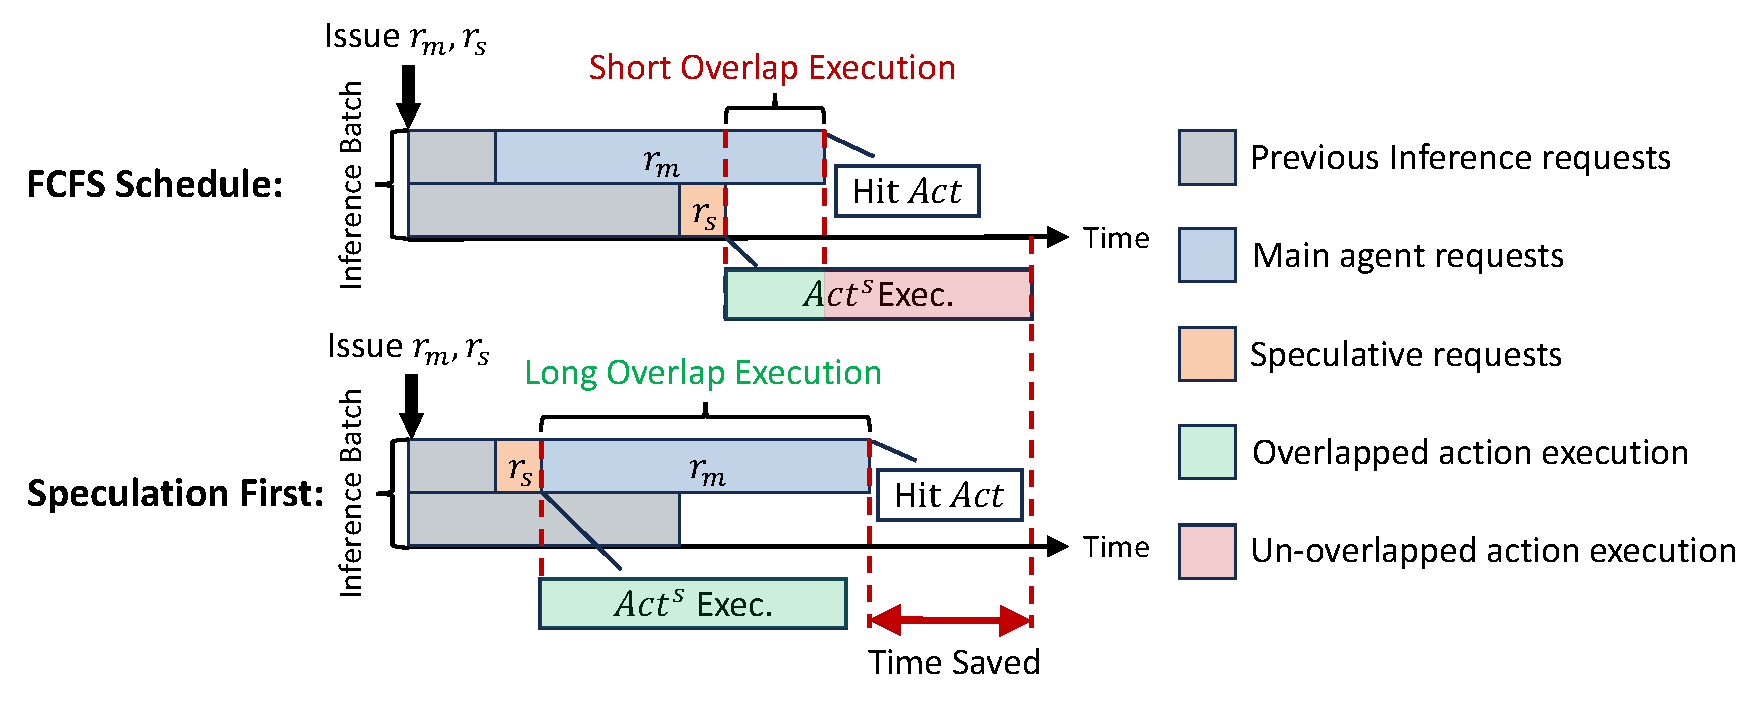
\includegraphics[width=0.98\linewidth]{figures/schedule.pdf}
    % \vspace{-10pt}
    \caption{Inter-Request Schedule between speculative requests and main agent requests.}
    % \vspace{-15pt}
    \label{fig:schedule}
\end{figure}

\subsection{Inter-Request Schedule}


Even with adaptive emission, speculation remains effective only if speculative requests complete before their corresponding main agent requests; otherwise, their results cannot be reused and the extra inference becomes pure overhead.
However, achieving this timing is non-trivial. 
Speculative and main agent requests have highly asymmetric output lengths: speculation typically produces fewer than ten tokens, while main agent reasoning may produce hundreds.
This asymmetry creates a system-level challenge that under a naive First-Come-First-Serve (FCFS) policy adopted by current inference engine, in which short speculative jobs may frequently queued behind long reasoning jobs, often completing only after they are no longer useful.

\system addresses this challenge through a speculation-first scheduling strategy inspired by Short-Job-First (SJF).
This design is motivated by two observations:
\begin{enumerate}[leftmargin=*]
    \item Speculative requests are extremely short.
    They typically generate fewer than ten tokens, while main agent reasoning may decode hundreds.
    Thus, their end-to-end latency is dominated by queuing delay, not computation.
    Prioritizing them yields disproportionate benefit, since it reduces queueing time without meaningfully delaying longer main agent requests.
    \item Verified speculation is only beneficial if speculative requests finish before its corresponding main agent request.
    In the Verified Speculation Phase, the speculative actions must be available before the main agent reasoning completes; otherwise, no overlap occurs.
    This induces a soft deadline that FCFS cannot satisfy, but SJF-style prioritization naturally does.
\end{enumerate}



As illustrated in \Figref{fig:schedule}, FCFS may cause a speculative request $r_s$ to begin long after its paired main agent request $r_m$, yielding only little overlap.
By contrast, prioritizing speculative requests ensures they begin early, enlarging the overlap window and reducing queuing delay for short jobs.
Even when a speculative action is incorrect, the resulting delay imposed on main agent requests remains minimal due to the tiny output size of speculative requests.
